\chapter{Introduction}
\label{chap:intro}

\section{Motivation}
\label{sect:motivation}
The performance of Lidar point clouds can be significantly affected by various weather conditions. For instance, in snowy weather, the presence of snowflakes on the surface can cause light reflections in different directions, leading to inaccuracies in the data. Similarly, in sunny weather, the shadows cast by vehicles can mimic the effects seen in rainy conditions, resulting in false predictions by the model. Additionally, camera images can encounter issues due to lens obstructions caused by rain or snow, which can lead to unclear or distorted visuals.

Moreover, foggy conditions can reduce the range and accuracy of Lidar sensors, as the dense particles in the air scatter the laser beams. This scattering effect can cause the Lidar to misinterpret the distance and shape of objects. Windy conditions can also introduce noise into the data, as moving debris or leaves can be mistakenly identified as obstacles.

Furthermore, the accumulation of snowflakes or water droplets on the Lidar sensor or camera lens can degrade the quality of the data collected. Regular maintenance and cleaning of these sensors are crucial to ensure optimal performance but It is not an easy job in  moving vehicle. 
\begin{figure}[!ht]
	\begin{minipage}[t]{.45\linewidth}
		
		
		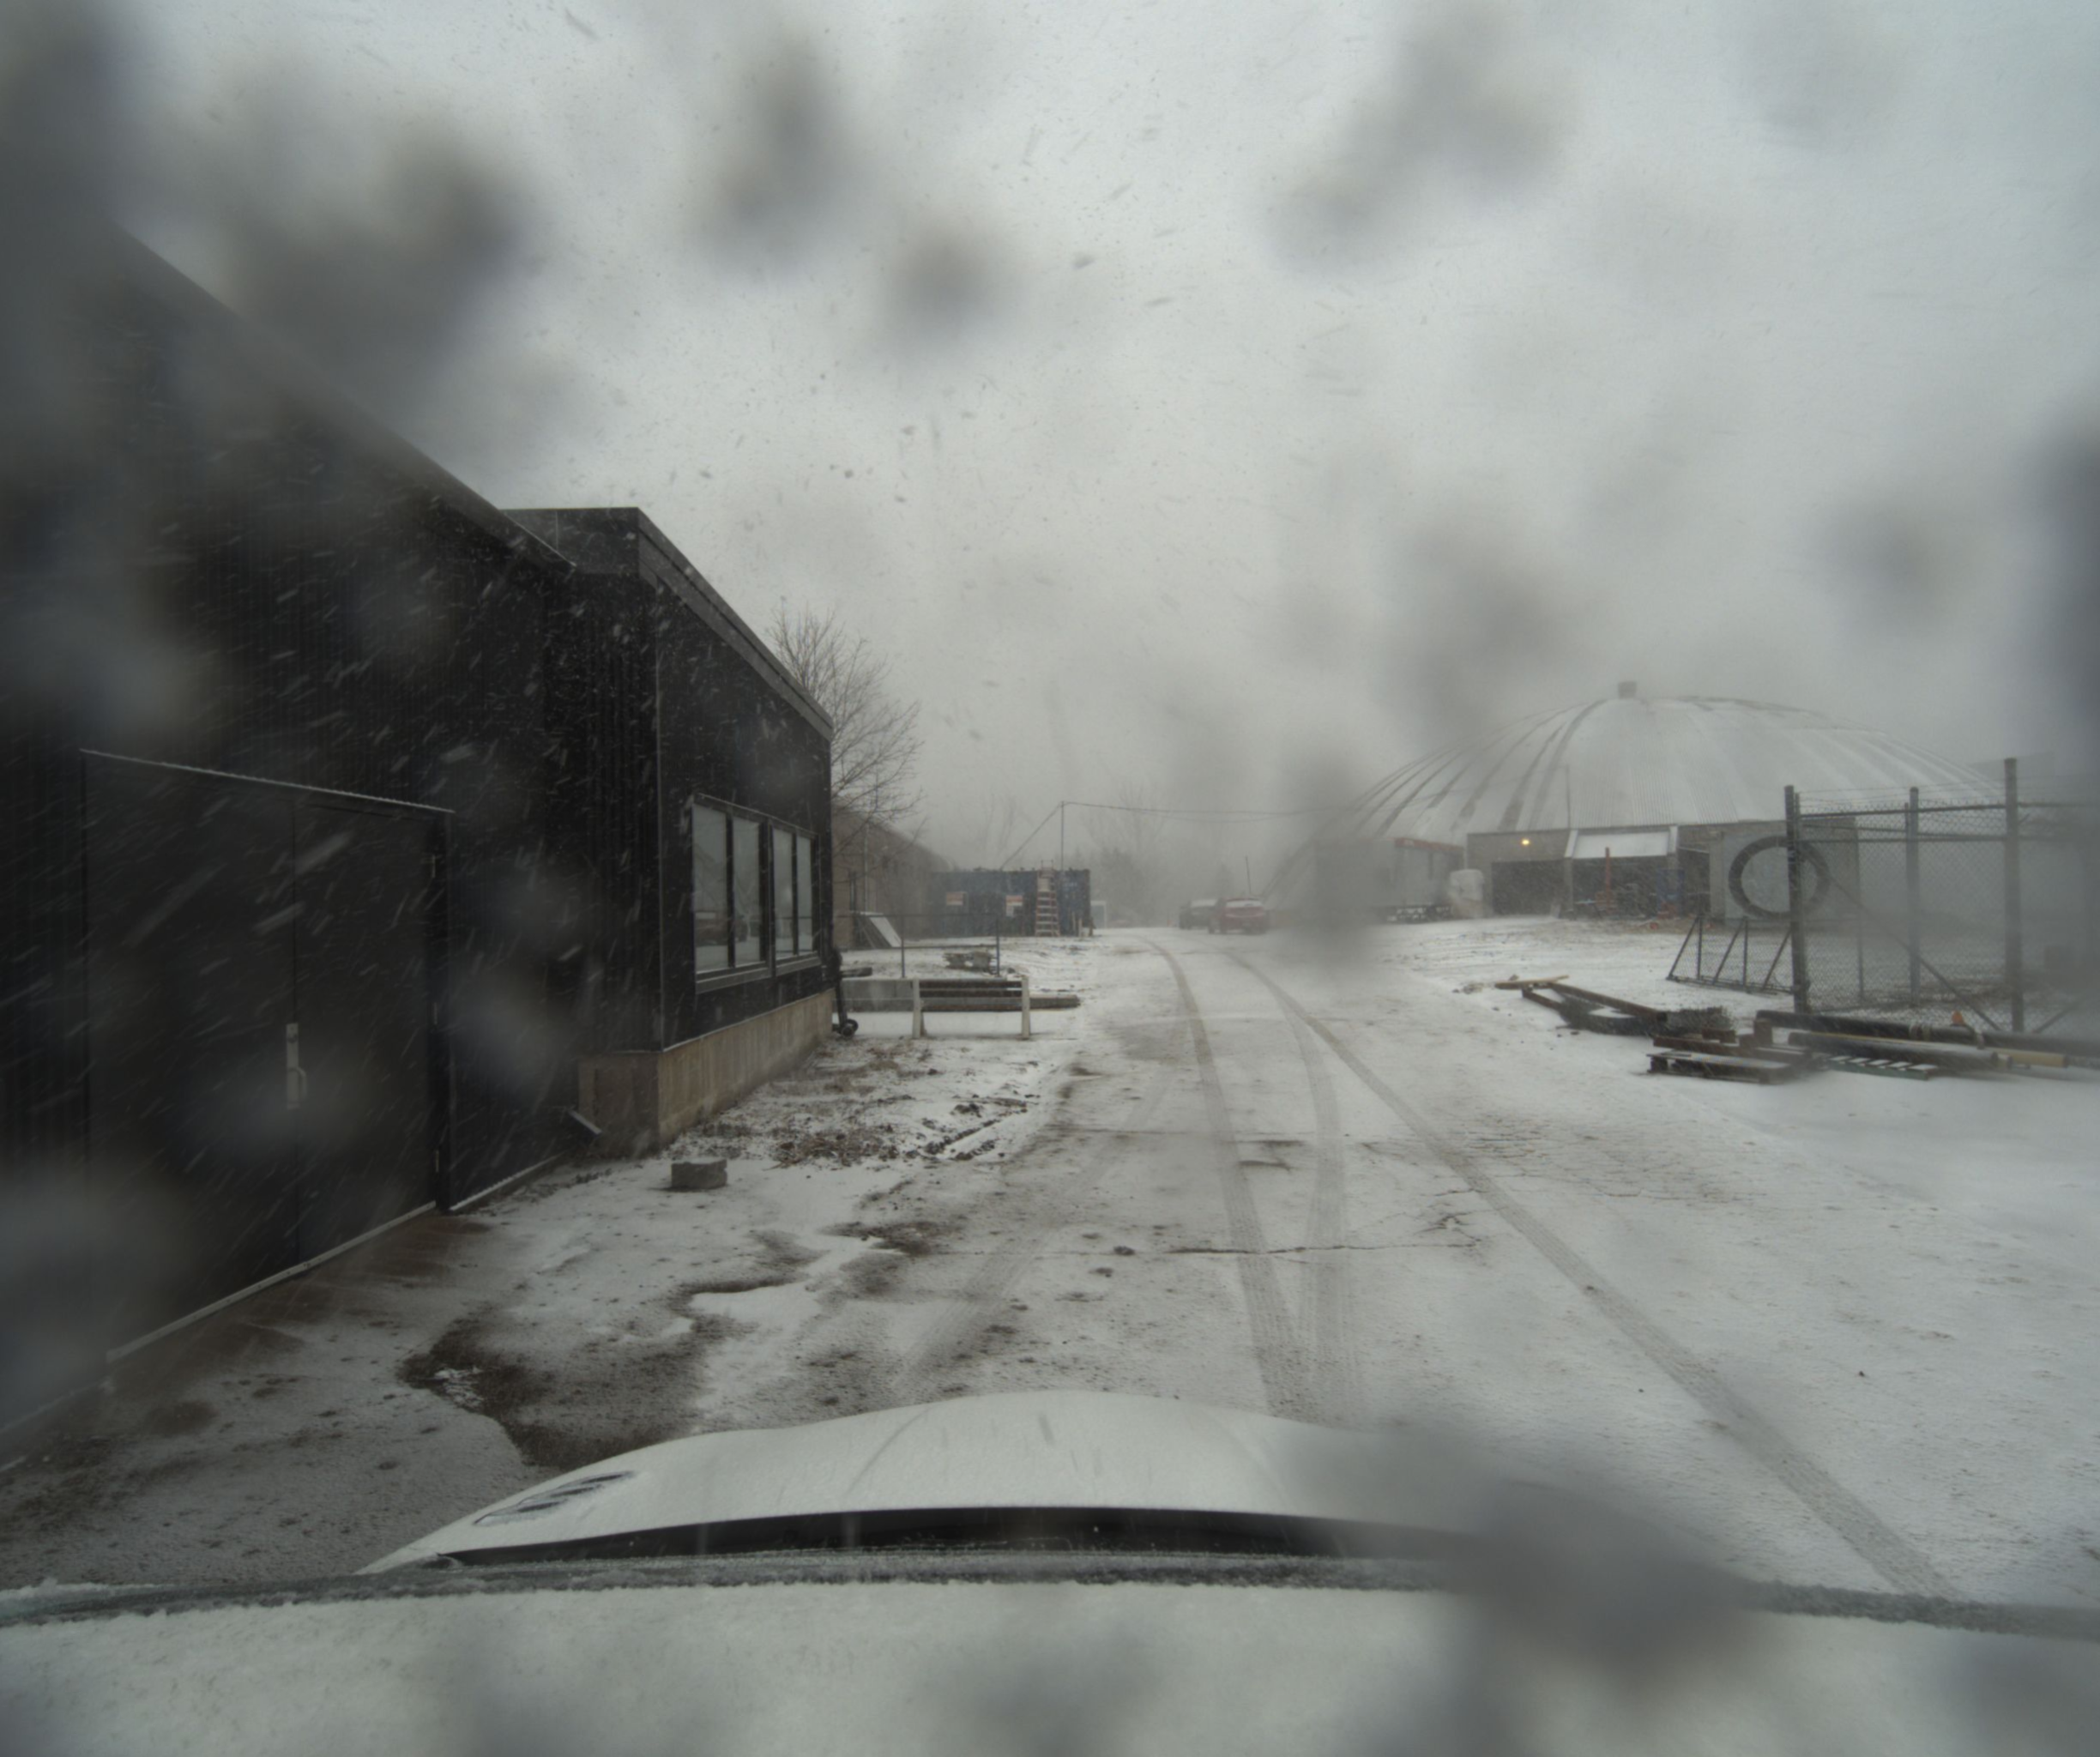
\includegraphics[width=\linewidth]{imgs/1611676774731026.png}
	\end{minipage}\hfill
	\begin{minipage}[b]{.45\linewidth}
		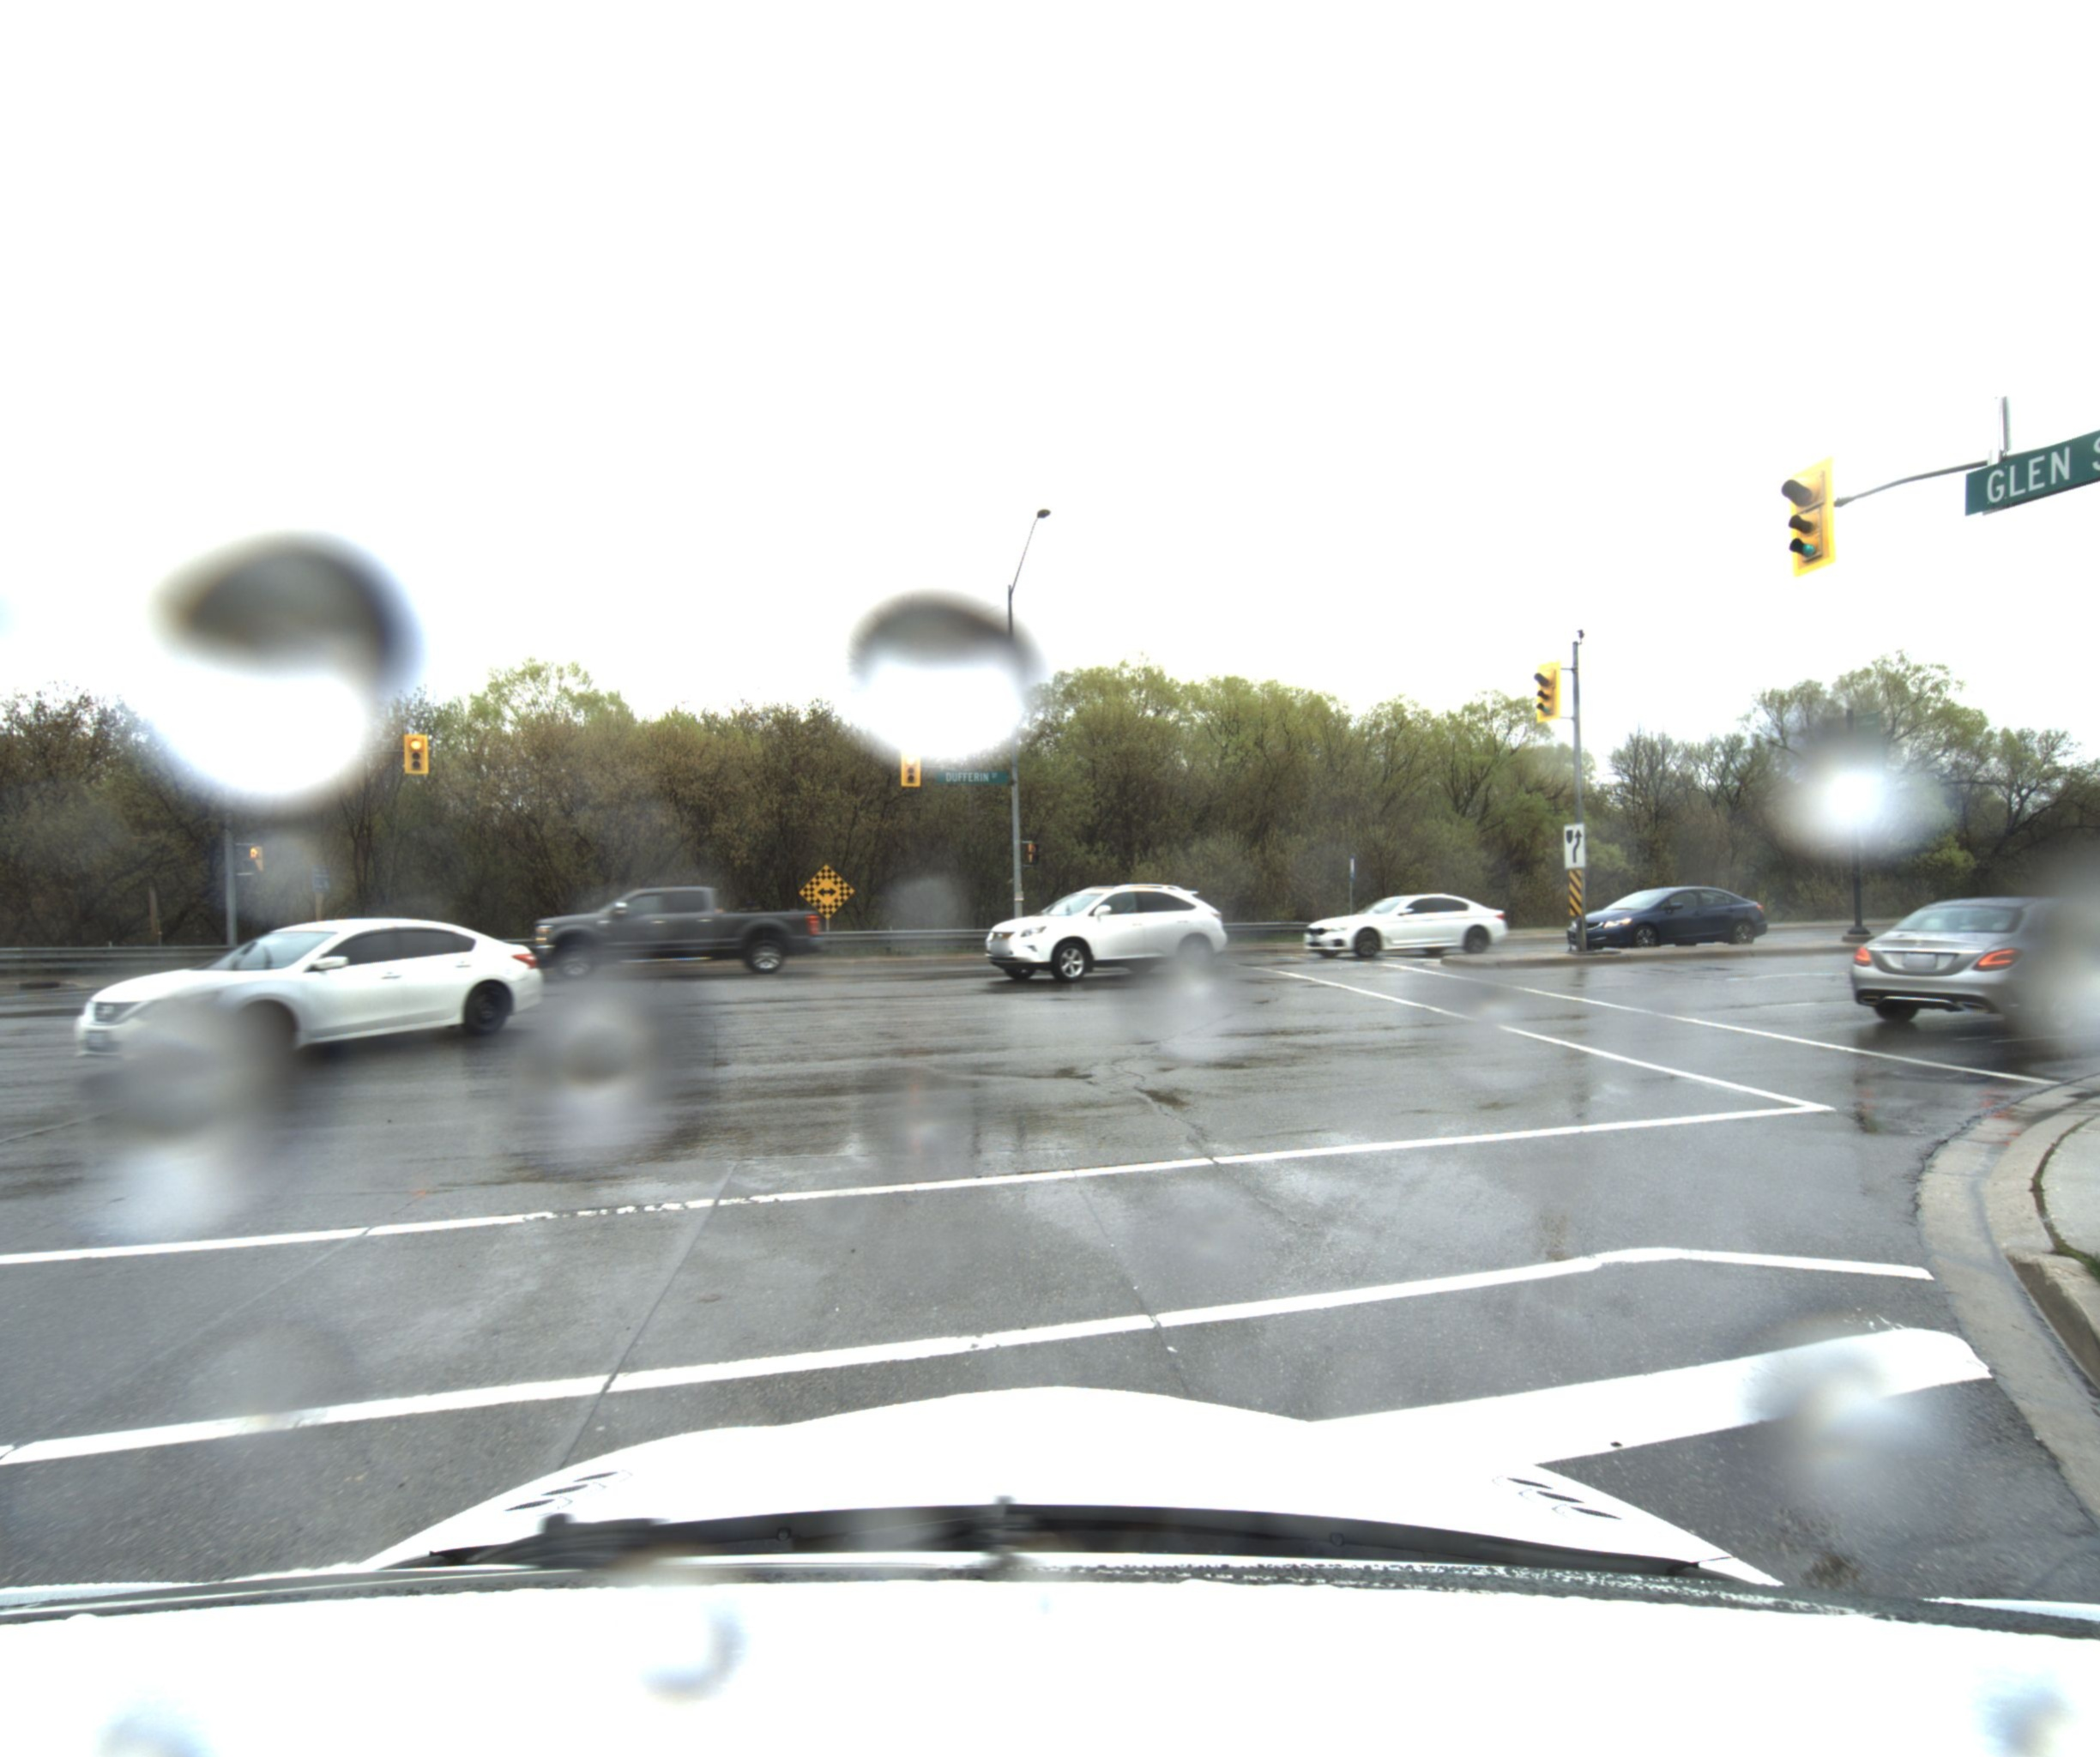
\includegraphics[width=\linewidth]{imgs/1619726918389964.jpg}
		
	\end{minipage}
	\caption{camera output in snow and rain weather conditions.}
	
	\label{img:rickety-camera}
\end{figure}

\section{Contributions}
Set up the Boreas dataset and modify the Pix2Pix and SPADE models to accept weather masks as input.
\section{Related Works}